	\section*{Problem 3}
	
	Let us consider what happens to $r_\parallel$ as $\theta_i$ goes from $0^\circ$ to $90^\circ$ for two ases, $n_i = 1$ and $n_t = 1.33$ and the 
	opposite. These two cases are displayed in the following two figures. Note Brewster's Angle is the angle such that 
	
	$$\theta_b = \theta_i + \theta_t = \frac{\pi}{2}$$
	
	\begin{figure}[!h]
		\centering
			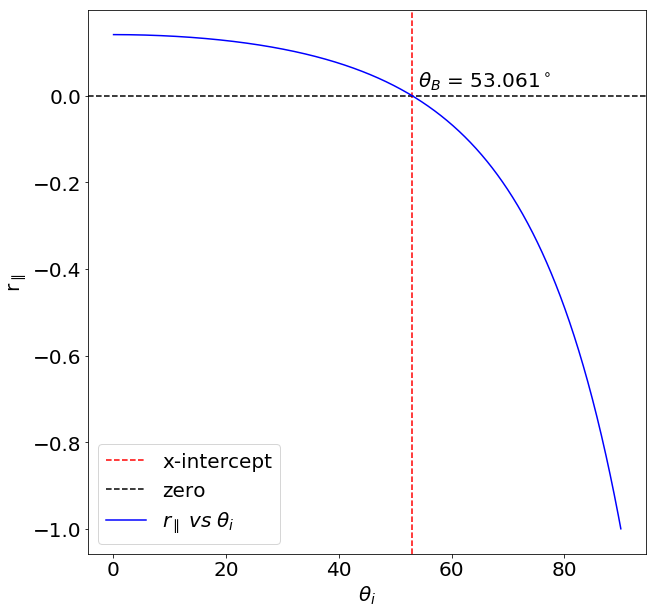
\includegraphics[width=0.75\textwidth]{r-par-1.png}
			\caption{Plot of $r_\parallel$ versus $\theta_i$ where $n_i > n_t$.}
	\end{figure}

	The above figure gives the plot we were looking for. Both it and the plot on the next page were calculated using python. As shown on the plot
	Brewster's Angle for the case where $n_i > n_t$ is $\theta_{brewster} = 53.1^\circ$.

	\begin{figure}[!t]
		\centering
			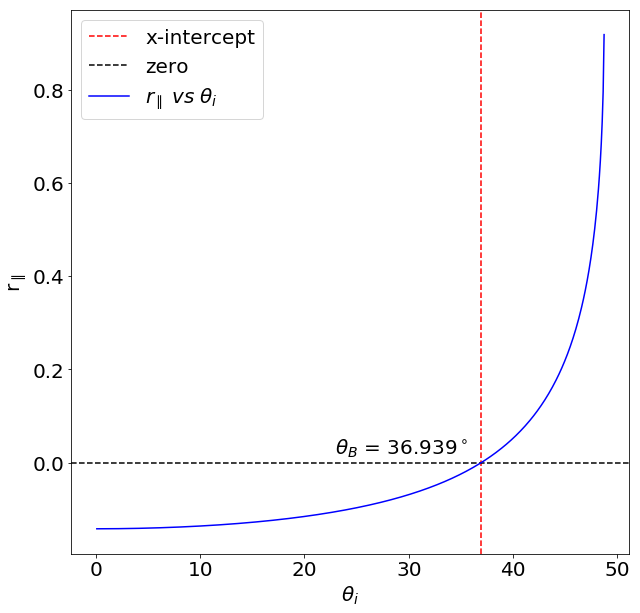
\includegraphics[width=0.75\textwidth]{r-par-2.png}
			\caption{Plot of $r_\parallel$ versus $\theta_i$ where $n_i < n_t$.}
	\end{figure}
	
	\pagebreak
	This figure shows that Brewster's Angle for the case $n_i < n_t$ is $\theta_{brewster} = 36.9^\circ$.
	These two plots give us the information we needed in order to solve Problem 3.